\section{研究内容及创新点}
\label{sec:intro:work}

\subsection{本文主要内容}
\label{sec:intro:work:mainwork}

随着VoLTE商用范围的扩大,研究VoLTE环境中构建时间隐通道,既扩充了时间隐通道构建方法,也扩展了对VoLTE音视频通话特征的研究。本文主要研究在VoLTE视频通话场景下,通过主动丢包的方式,构建鲁棒的时间隐通道。主要包括四个研究点,分别为面向VoLTE中主动丢包时间隐通道的检测方法研究、基于Zigzag映射矩阵的时间隐通道构建方法研究、基于多重校验的时间隐通道构建方法研究,以及基于Linphone的时间隐通道构建方法验证。各部分与研究指标的关联关系如图\nref{fig:1:contents}。

\insertFigure{
	\begin{figure}[htbp]
		\centering
        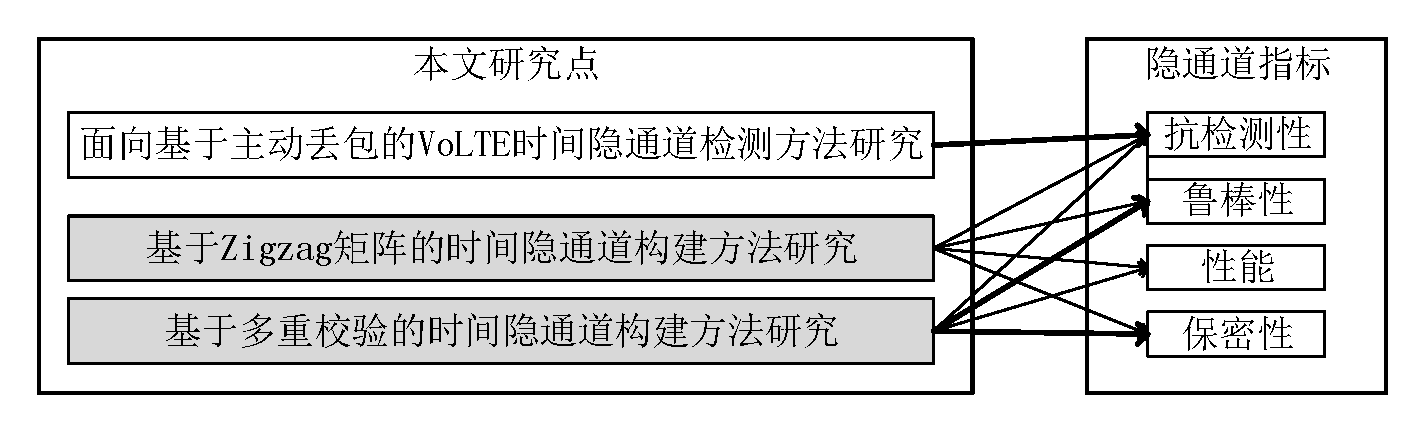
\includegraphics[width=0.95\textwidth]{chapters/chapter1/figures/struct.pdf}
        \caption{本文研究点与时间隐通道指标的对应关系}\label{fig:1:contents}
	\end{figure}
}

%背景介绍了什么
背景及相关工作部分,主要介绍了本文主要工作对应的研究基础,以及国内外研究现状。内容包括VoLTE音视频传输方案的分析,分析了实际商用中数据采集、处理、传输、呈现流程,并分析了音视频处理流程的差异。对现有时间隐通道构建方案的分析,涵盖了以太网中的构建方案、移动互联网下的构建方案,以及常用的鲁棒性策略。通过分析VoLTE传输协议,研究丢包对传输过程产生的影响,并分析协议中有效的随机字段。抗检测能力是时间隐通道的重要指标,通过分析现有的时间隐通道检测方法,研究可用于检测主动丢包时间隐通道的方法。

%检测方法介绍了什么
面向VoLTE中主动丢包时间隐通道的检测方法研究,主要研究在VoLTE场景下,如何有效检测基于主动丢包的时间隐通道。为筛选有效的检测模式,首先分析VoLTE通话抓包结果,包含丢包率、IPD、突发丢包长度及区间丢包数几个方面。根据分析结果,总结出了基于统计分析的时间隐通道检测方法,包含不同维度的多种检测方式。最后,通过模拟测试,验证隐通道检测方法。

%Zigzag方法说了什么
基于Zigzag映射矩阵的时间隐通道构建方法研究,研究利用Zigzag矩阵构建时间隐通道,同时在抗检测性、鲁棒性及传输性能之间实现均衡。按照研究背景和动机、构建方法介绍及评估结果的顺序,对该方法的研究基础、架构设计、调制解调方法及实验测试结果分别进行介绍。经过实验测试证明,通过调整传输参数,该时间隐通道达到了设计要求,具有良好的测试表现。

%多重校验方法说了什么
基于多重校验的时间隐通道构建方法研究,重点研究如何进一步降低误码率,提高传输鲁棒性。在该时间隐通道方法中,设计了包括码字间校验、码字自校验以及符号校验三级校验模式,结合不同规模的映射矩阵,显著提高了鲁棒性。该部分首先由研究背景开始,然后介绍该方法的设计架构,接下来逐层展开核心的鲁棒性方法。最后实验结果表明,该时间隐通道的鲁棒性有了大幅度提升。

%Linphone中验证说了什么
基于Linphone的时间隐通道构建方法验证,通过实际传输测试,检验主动丢包方法是否符合规范。基于主动丢包的时间隐通道,调制过程的最后阶段为主动丢包,本部分验证其有效性。该验证基于Linphone平台,添加了UI层的隐通道控制接口、SDK层的消息传输接口,以及oRTP层的隐通道执行组件。通过实际传输测试验证,基于主动丢包的时间隐通道数据传输模式有效,传输方式切实可行。

%以上各部分是怎样在逻辑上串起来的
背景及相关工作的介绍,分析出在VoLTE视频通话场景下,通过主动丢包的方式构建时间隐通道是可行的。与此同时,现有的检测方法及鲁棒性方法,无法有效覆盖这种隐通道构建模式。面向VoLTE中主动丢包时间隐通道的检测方法研究,着重解决如何检测采用主动丢包的时间隐通道,同时也为本文提出的构建方案提供检测依据。接下来,提出了两种不同的时间隐通道构建方法,分别从不同的方式,填补鲁棒性方面的需求,并通过实验进行验证。最终,在Linphone平台中对主动丢包方法进行传输测试,验证主动丢包方式实际可行,从而本文中的时间隐通道构建方法均具有可行性。

\subsection{本文主要创新点}
\label{sec:intro:work:inno}

本文的研究重点,是在VoLTE场景下,通过主动丢包方式构建时间隐通道,以及抗检测性评估方式。主要的创新点包括以下四点:

\begin{enumerate}
    \item 提出了一种VoLTE场景中,对基于主动丢包时间隐通道的检测方法。该方法以统计分析为基础,综合多种量化评估方法,结合IPD及丢包特征两个维度进行检测判别。传统的时间隐通道检测方法,主要基于IPD分布进行检测识别,对基于主动丢包的时间隐通道来说,判别效果不够全面。本方法完善了时间隐通道的检测方式,经过实验测试,该时间隐通道检测方法能够检测出主动丢包率高于{0.4\ \%}的时间隐通道。
    \item 提出了一种基于Zigzag映射矩阵的时间隐通道构建方法,通过在编码过程中添加CRC校验信息,并利用Zigzag矩阵建立码字到符号的转换。该方法具有简单高效的设计,以轻量级校验模式,在保证传输性能的同时,降低计算复杂度保证鲁棒性。实验结果表明,该方法具有良好的抗检测能力,传输性能可达到{0.88\ bps},误码率保持在{1.5\ \%}左右,同时具有极低的构建代价。
    \item 提出了一种基于多重校验的时间隐通道构建方法,重点研究如何通过逐级校验的方式,降低噪声对时间隐通道的干扰。该方法的核心,是在不同的处理阶段引入相互独立的校验方式,在解调过程中逐级剔除噪声干扰,还原概率最高的隐蔽消息。此外,通过引入可调映射矩阵,将连续丢包事件分散处理,减小每组的噪声强度。经过实验测试,该方法在保持传输速率为{0.49\ bps}时,误码率不高于{0.08\ \%},在鲁棒性方面得到显著提升。
    \item 基于Linphone平台,验证了基于主动丢包的时间隐通道构建方法。Linphone与VoLTE采用相同的SIP(Session Initiation Protocol)+RTP通话模式,通过在Linphone中构建基于主动丢包的时间隐通道,证明该构建模式符合VoLTE网络环境约束,时间隐通道传输能力有效。
\end{enumerate}

\subsection{本文组织结构}
\label{sec:intro:work:struct}

全文共分五章,文章的组织结构如下:
\begin{itemize}
    \item 第1章,对本文的研究领域及主要内容进行介绍。
    \item 第2章,介绍本文中涉及的研究背景,及国内外相关工作。内容包含当前工作的研究基础,当前隐通道构建及检测方面的研究成果,以及时间隐通道应当满足的基本要求。
    \item 第3章,介绍面向VoLTE中主动丢包时间隐通道的检测方法,通过结合多种特征及多种检测工具的结果,提高隐通道检测能力。检测模式涵盖了基于统计曲线的检测、基于熵的检测及基于相对距离的检测方法,能够对基于主动丢包的时间隐通道进行有效识别。该检测方法,也是本文中时间隐通道构建方法抗检测能力的评估方法。
    \item 第4章,介绍基于Zigzag映射矩阵的时间隐通道构建方法,包含研究背景和动机、整体设计方案、实验及评估结果几部分。
    \item 第5章,介绍基于多重校验的时间隐通道构建方法,包含背景和动机、隐通道整体设计方案、各层次鲁棒性方法,以及实验测试评估结果几部分。
    \item 第6章,介绍基于Linphone的时间隐通道构建方法验证,包含Linphone的基本结构、添加的模块以及关联关系,以及传输测试结果几部分。
\end{itemize}